\begin{appendices}
\chapter{L'ajout de points}

\label{Annexe1}
\begin{java}[L'ajout de point à un trajet]  
public void addLocation(Location l) {
	//Si il n'y a pas de points d'enregistres
	if (locations.size() == 0) {
		distance = 0;
		locations.add(l);
		temps = 0;
	} else {
	
	//On recupere la derniere position 
	Location last = getLastPosition();
	
	//On augmente la distance total du trajet 
	distance += last.distanceTo(l);
	locations.add(l);
 	
 	//On incremente egalement le temps 
	if (locations.size() == 1) {
		temps = 0;
	} 
	temps += ((l.getTime() / 1000) - (last.getTime() / 1000));   
	}
}
\end{java}

\chapter{Calcul de la distance entre deux points}
\label{Annexe2}

\chapter{Les providers Android}
\label{Annexe3}
\begin{center}
   \begin{tabular}{| c | c | l | }
     \hline
     Accuracy & Power Usage & Technology \\ \hline
     20ft & High & Autonomous GPS, Provider: gps \\ 
     && uses GPS chip on the device \\
     && line of sight to the satellites \\
     && need about 7 to get a fix \\
     && takes a long time to get a fix \\
     && doesn’t work around tall buildings \\ \hline
 
     200ft & Medium & Assisted GPS (AGPS), Provider: network \\ 
     && uses GPS chip on device, as well as assistance from the network to provide a fast initial fix \\
	 && very low power consumption \\
	 && very accurate \\
	 && works without any line of sight to the sky \\
	 && depends on carrier and phone supporting this \\ \hline
    
    1 mile & Low & CellID lookup/WiFi MACID lookup, Provider: network or passive \\
     && very fast lock, and does not require GPS chip on device to be active \\
	 && requires no extra power at all \\ 
     && has very low accuracy \\
     \hline
   \end{tabular}
 \end{center}
	 	
		

		

		

\footnote{\href{http://developerlife.com/tutorials/?p=1375}{developerlife}}

\chapter{Captures d'écrans de l'application}
\label{Annexe3}
\begin{multicols}{3}
\begin{img}
  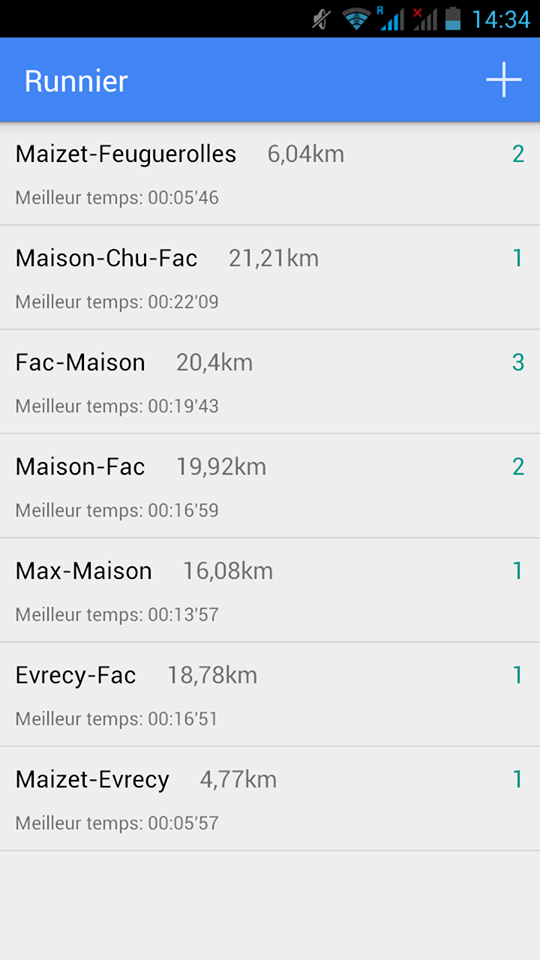
\includegraphics[scale=0.3]{img/home.jpg}
  \caption{Liste des parcours}
\end{img}
\begin{img}
  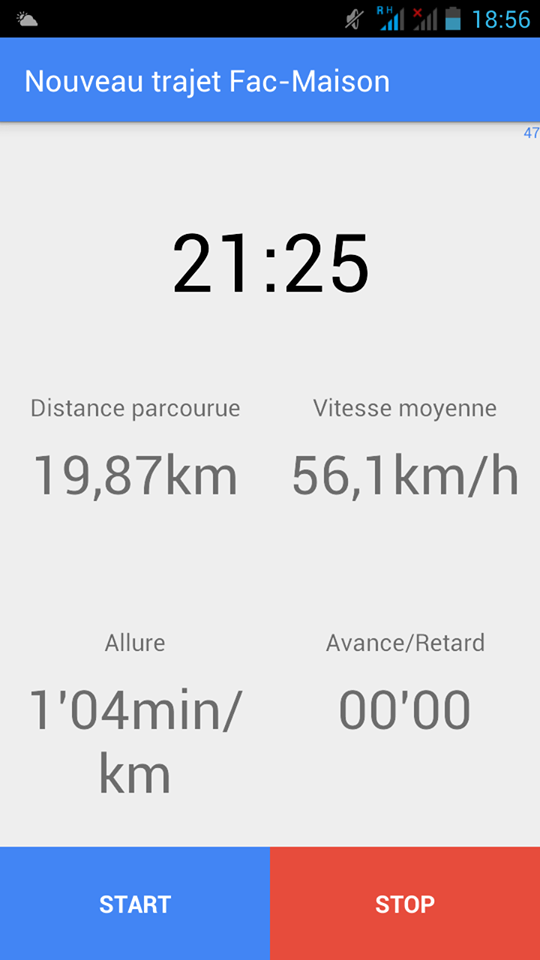
\includegraphics[scale=0.3]{img/direct.jpg}
  \caption{Enregistrement d'un trajet}
\end{img}
\begin{img}
  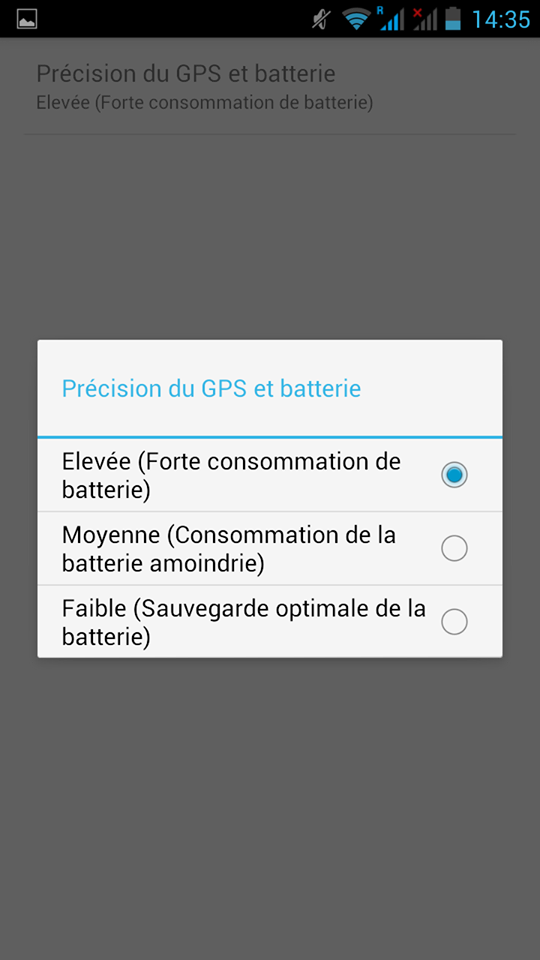
\includegraphics[scale=0.3]{img/parametres.jpg}
  \caption{Paramètres}
\end{img}
\end{multicols}

\end{appendices}


